% !TEX encoding = UTF-8 Unicode
% !TEX root = thesis-ex.tex

This section discusses the measurement of the inclusive jet \RAA\ as measured by the ALICE detector for jets in $\sqrtsnn=2.76$ TeV \pbpb\ and \pp\ collisions \cite{Reed_2013}.

While measurements that compare jets in a dijet system to each other as discussed in Section~\ref{sec:xj} can provide valuable information about how jets lose energy, they have the following limitation: If both jets lose equal amounts of energy, the dijet yield will still be peaked at unity and no new information will be obtained.
Thus, it is useful to compare the jet yields directly between the \pp\ and \pbpb\ systems and construct the jet \RAA\ observable.
This is defined as:

\begin{align}
\RAA  = \dfrac{\dfrac{1}{N_{\rm evt}} \left.
\dfrac{d^2 N_{\rm jet}}{d\pt dy} \right|_{\rm cent}}{ \langle T_{\rm AA} \rangle \left.
\dfrac{d^2\sigma_{\rm jet}}{d\pt dy} \right|_{\rm pp}}
\end{align}
where \TAA\ is the nuclear thickness function and accounts for the geometric enhancement between \pp\ and \pbpb\ as discussed in Section~\ref{sec:HICollisions} and \cite{doi:10.1146/annurev.nucl.57.090506.123020}.

The jet spectrum in \pbpb\ events, as well as the jet \RAA\ for central \pbpb\ is shown in Figure~\ref{fig:jet_raa_alice}.
\begin{figure}[htbp]
\begin{center}
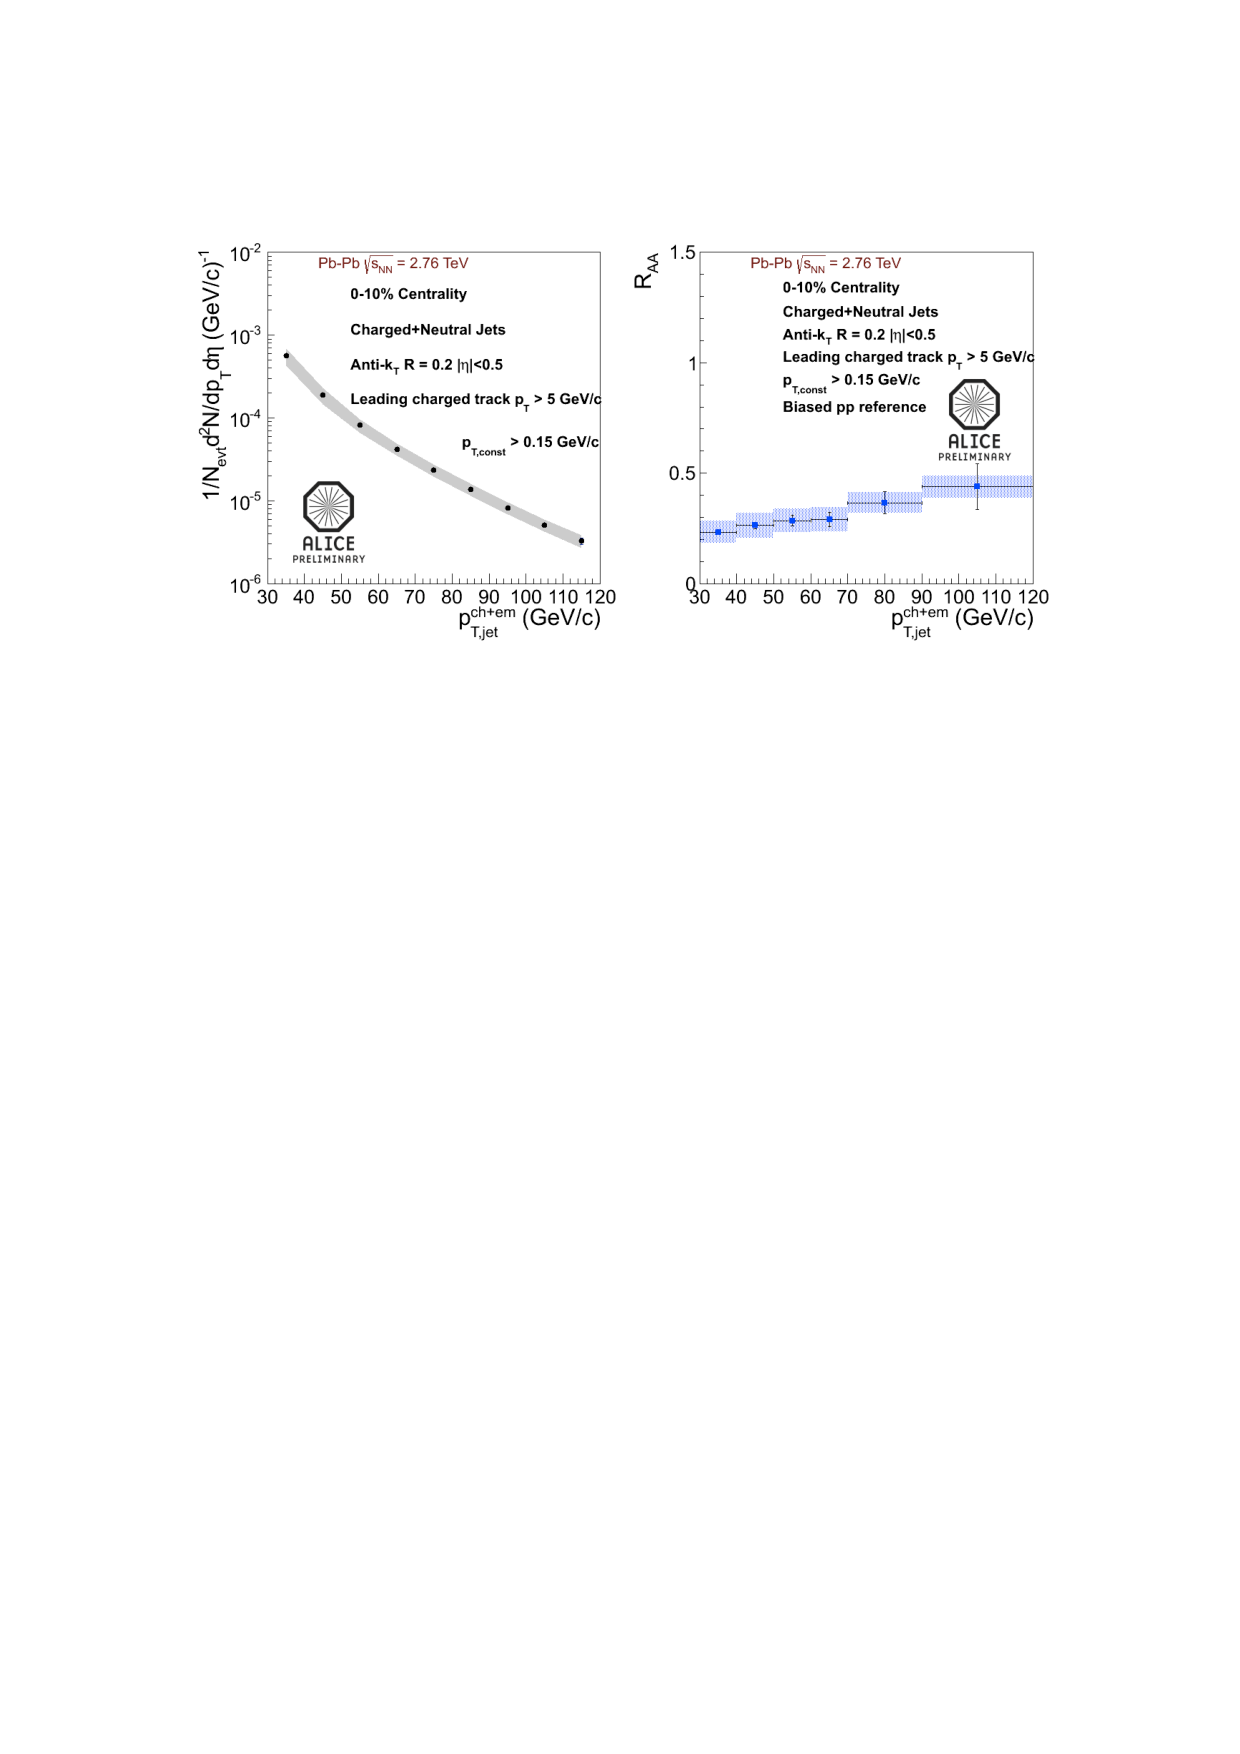
\includegraphics[width=0.85\textwidth]{figures/jetMeasurements/jet_raa_alice}
\caption{(Left) The inclusive jet cross section as a function of jet \pt\ in 0--10\% central \pbpb\ collisions at $\sqrtsnn = 2.76$ TeV.
The band around the data points represents the systematic uncertainty.
(Right) The \RAA\ for 0--10\% central \pbpb\ collisions.
Figure taken from \cite{Reed_2013}.}
\label{fig:jet_yields}
\end{center}
\end{figure}

It can be seen that the most central collisions show a clear suppression with an $\RAA \approx 0.25$ at jet $\pt\ 30$ GeV.
The \RAA\ value slowly evolves with jet \pt\ and rises to 0.5 at jet $\pt = 100$ GeV.
This modification becomes smaller for more peripheral collisions.

These observations are consistent with results from ATLAS and CMS \cite{Aad:2014bxa, 2019108, Khachatryan:2016jfl}.
The ATLAS results at $\sqrtsnn = 5.02$ TeV are shown in Figure~\ref{fig:jetraa_atlas}.
The higher collision energy allows access to higher \pt\ jets.
The smooth centrality dependence can be more clearly seen in Figure~\ref{fig:raa_centDep_atlas}, where \RAA\ is shown as a function of \ANpart\ for jets the 100--126 GeV and 200--251 GeV ranges.
The magnitude of the suppression is also seen to significantly depend on jet \pt\ for $\ANpart \geq 50$.


%This measurement was conducted for jets in the 40--1000 GeV range in different rapidity and centrality intervals.
%The jet yields in \pp\ and \pbpb\ collisions are shown in Figure~\ref{fig:jet_yields} .
%The \pbpb\ jet yields are scaled by the thickness function and are shown for 8 centrality intervals.
%\begin{figure}[htbp]
%\begin{center}
%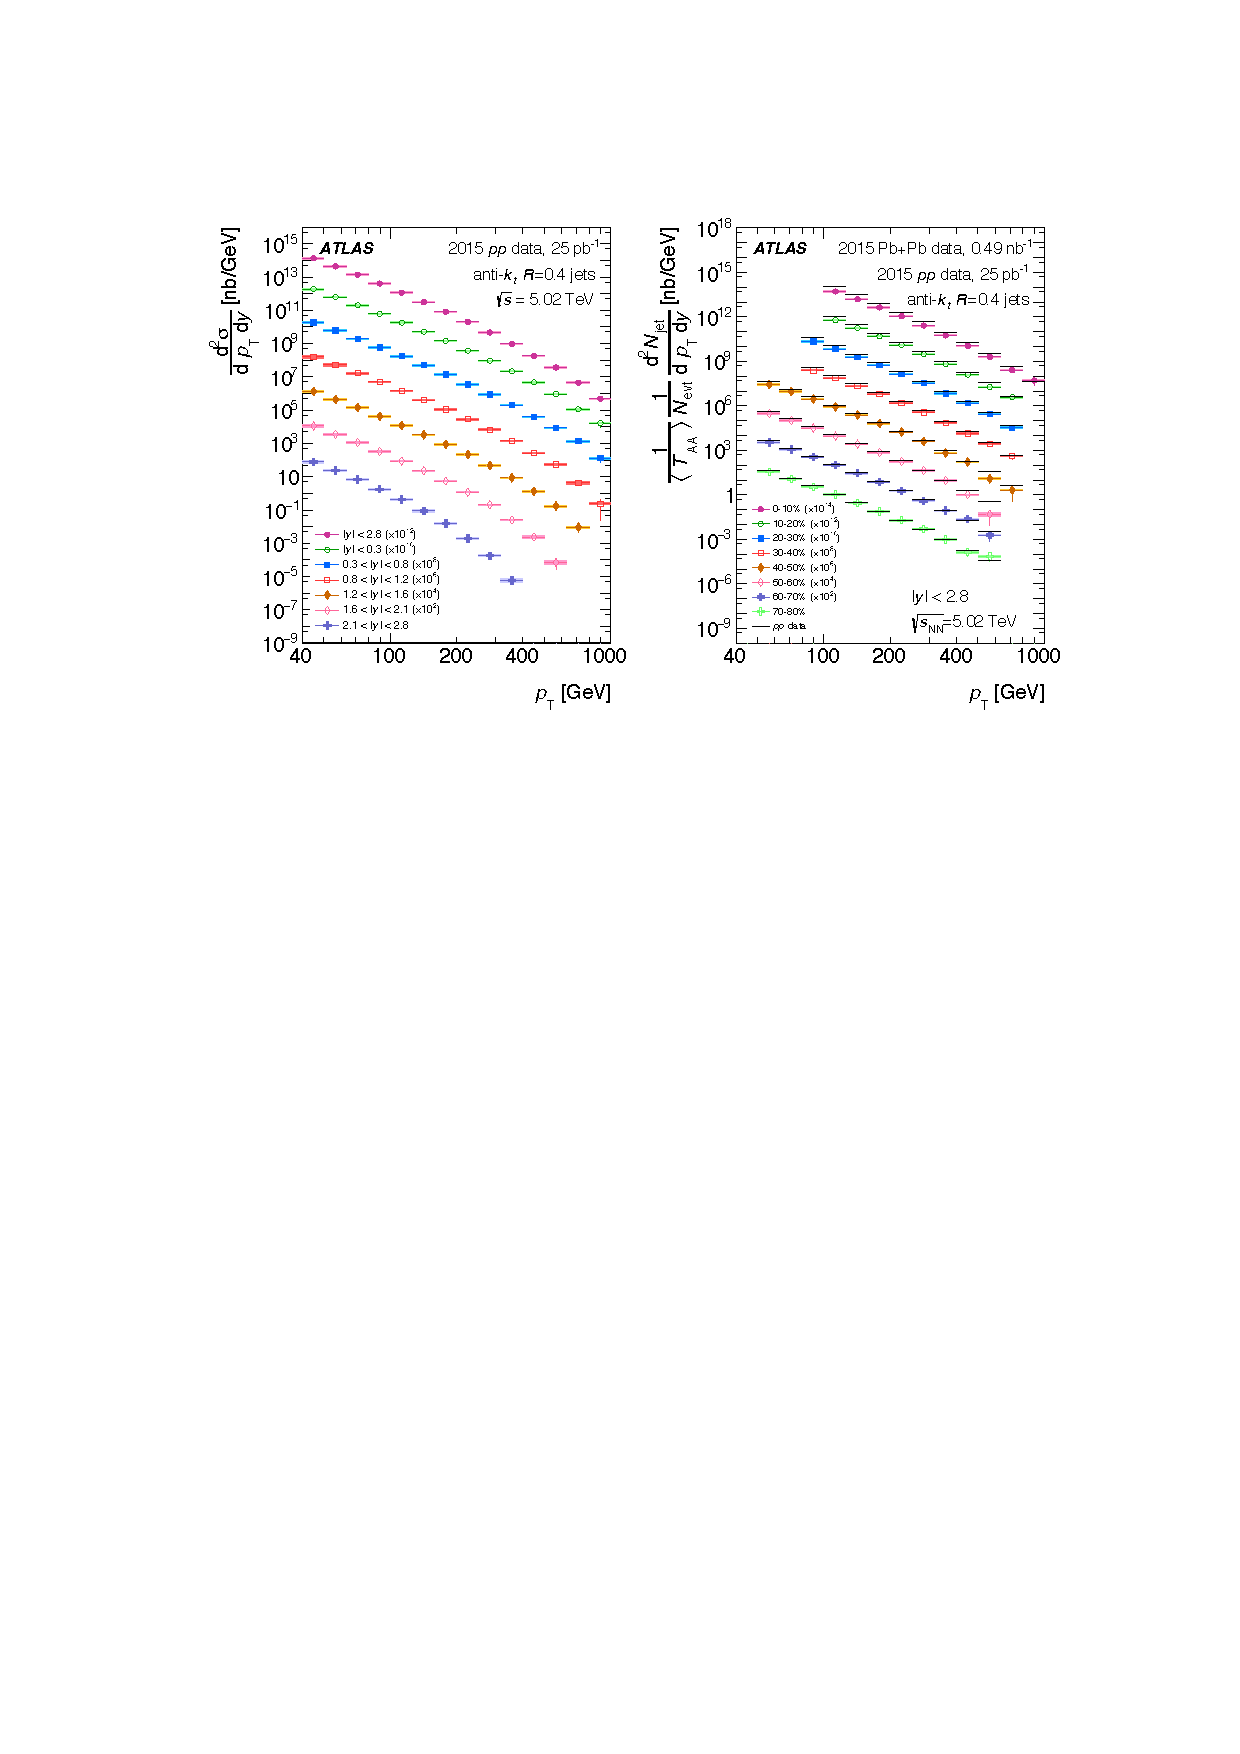
\includegraphics[width=0.85\textwidth]{figures/jetMeasurements/jetYields}
%\caption{(Left) The inclusive jet cross section in \pp\ collisions as a function of jet \pt\ in different $|y|$ intervals scaled by successive powers of $10^2$ for visibility.
%(Right) Per event inclusive jet yield in \pbpb\ collisions normalized by $\langle \TAA \rangle$ as a function of jet \pt\ in different centrality intervals scaled by successive powers of $10^2$ for visibility.
%The solid lines represent the cross section from \pp\ data at the same rapidity interval scaled by the same $10^2$ factor.
% Figure taken from \cite{2019108}.}
%\label{fig:jet_yields}
%\end{center}
%\end{figure}
%Figure~\ref{fig:raa} shows the measured inclusive jet \RAA\ as a function of jet \pt\ for different centrality bins and jet rapidity $|y| < 2.8$.
%It can be seen that the most central collisions show a clear suppression with an $\RAA \approx 0.45$ at jet $\pt\ 100$ GeV.
%The \RAA\ value slowly evolves with jet \pt\ and rises to 0.6 at jet $\pt = 800$ GeV.
%This modification becomes smaller for more peripheral collisions.




\begin{figure}
\begin{subfigure}{.45\textwidth}
  \centering
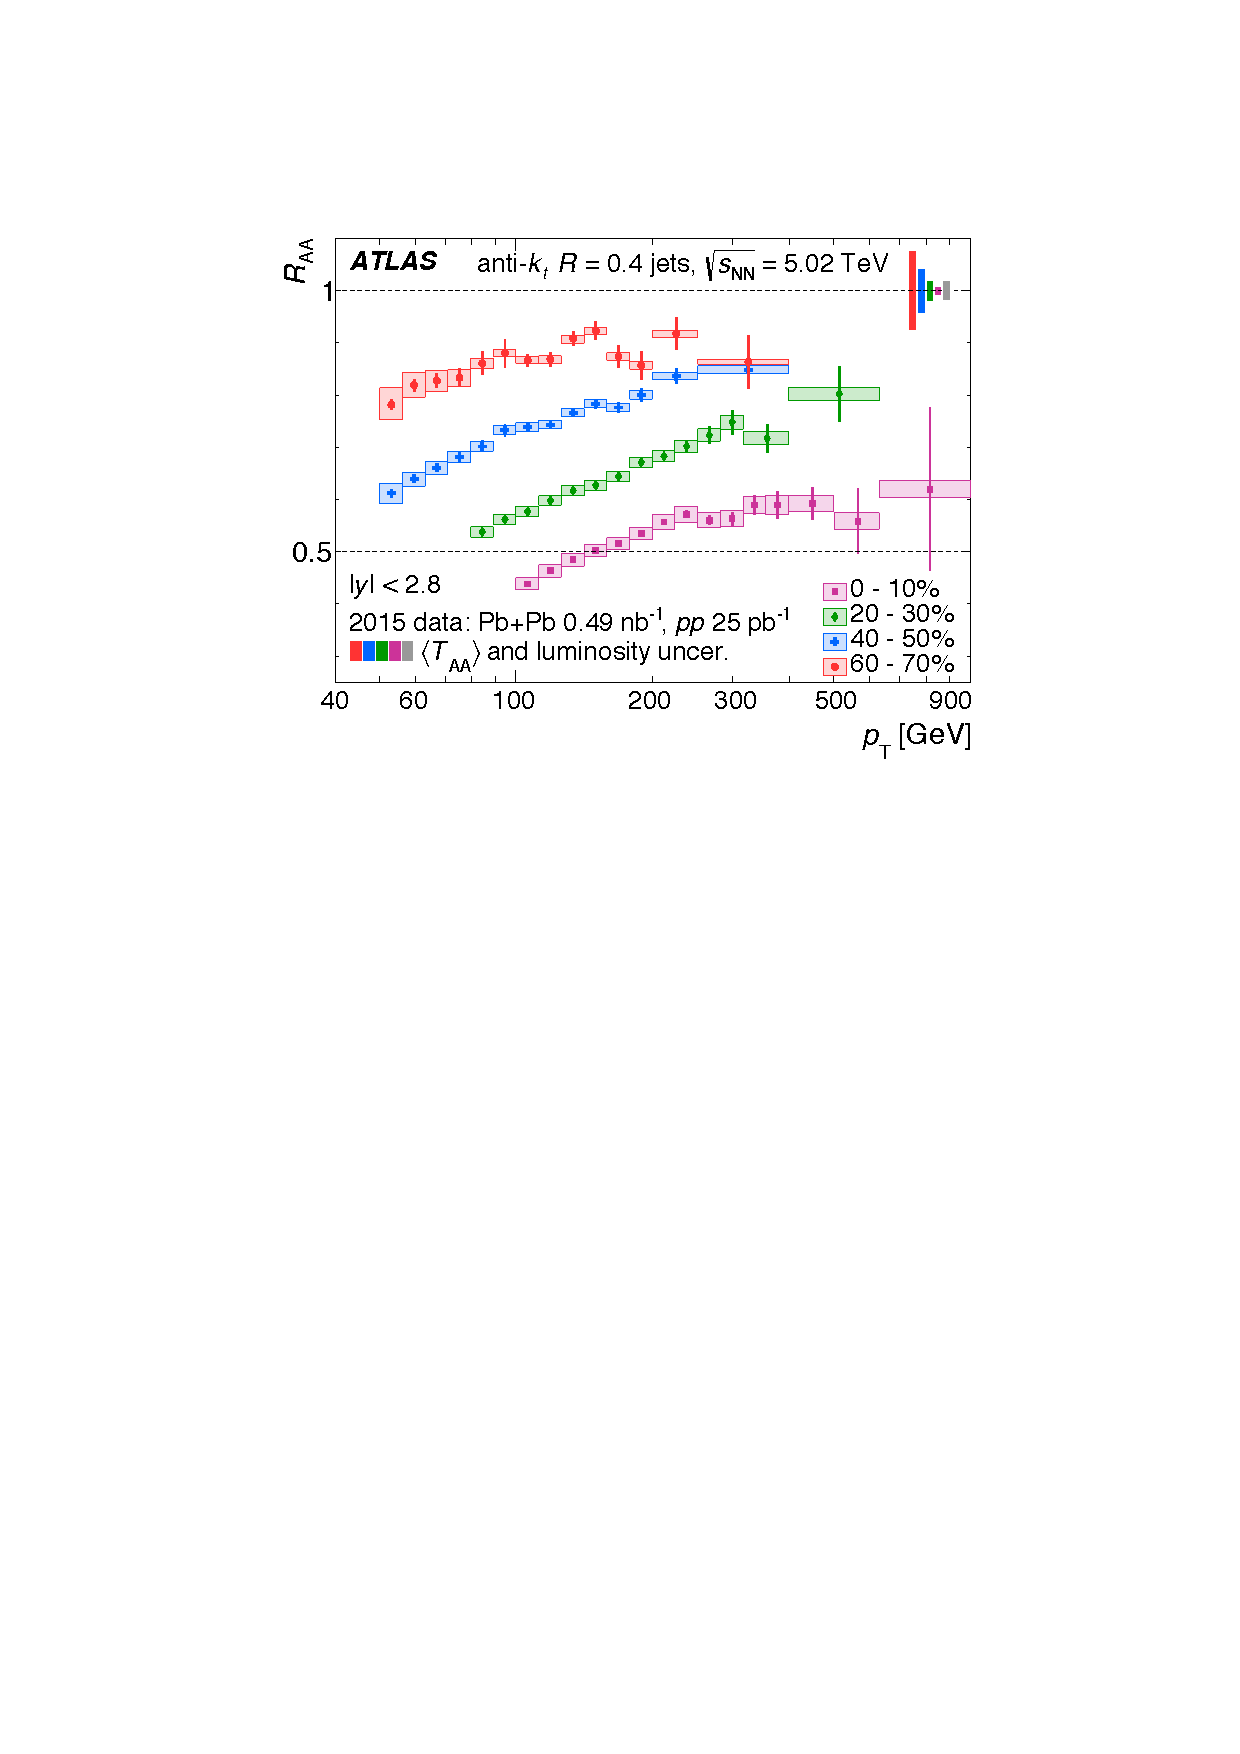
\includegraphics[width=\textwidth]{figures/jetMeasurements/raa}
\caption{}
\label{fig:jetraa_atlas}
\end{subfigure} \qquad
\begin{subfigure}{.45\textwidth}
  \centering
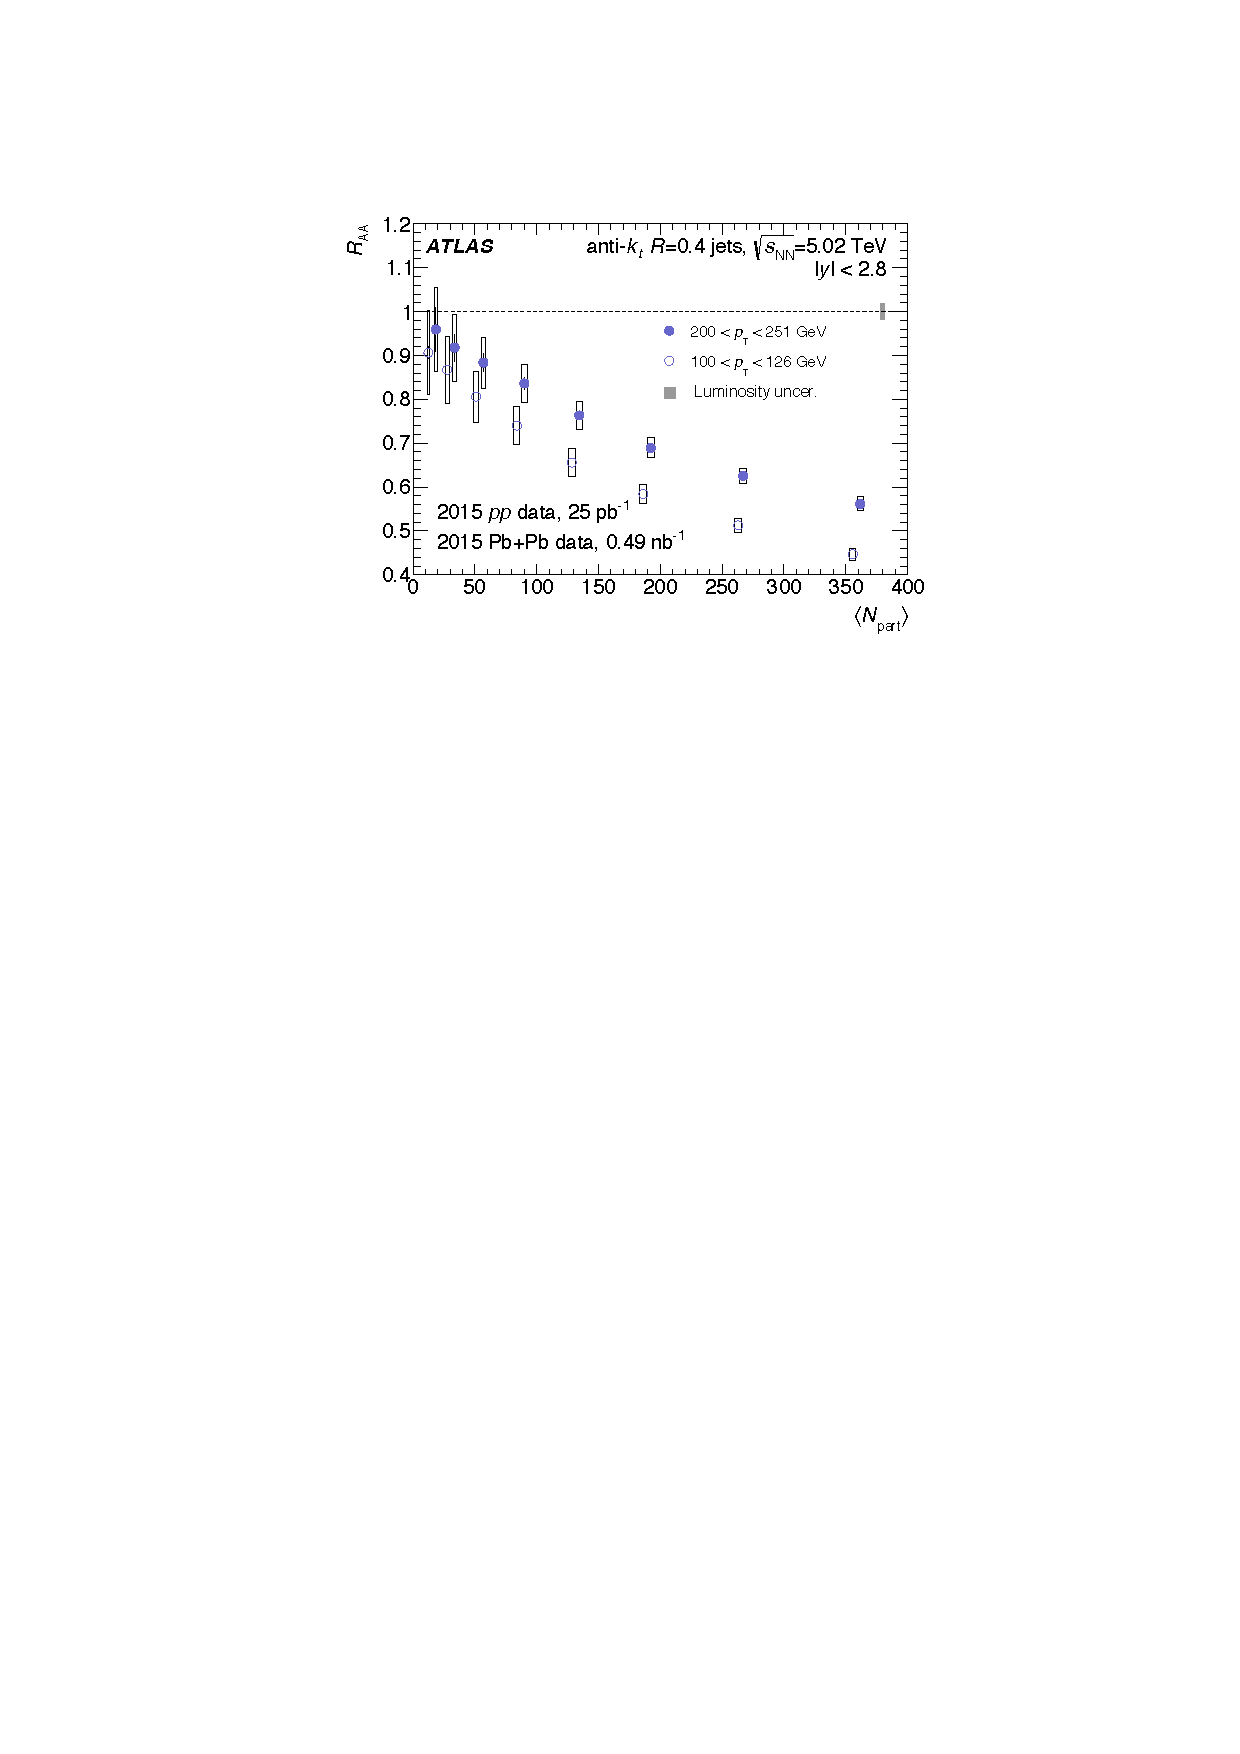
\includegraphics[width=\textwidth]{figures/jetMeasurements/raa_centDep}
\caption{}
\label{fig:raa_centDep_atlas}
\end{subfigure}
\caption{(Left) The \RAA\ distributions as a function of jet \pt\ for different centrality bins and jet rapidity $|y| < 2.8$.
(Right) The \RAA\ distributions as a function of jet $\langle \Npart \rangle$ for different jet \pt\ bins and jet rapidity $|y| < 2.8$.
Figures taken from \cite{2019108}}
\label{fig:atlas_jet_raa}
\end{figure}

%
%\begin{figure}
%\begin{center}
%  \begin{minipage}[b]{0.43\textwidth}
%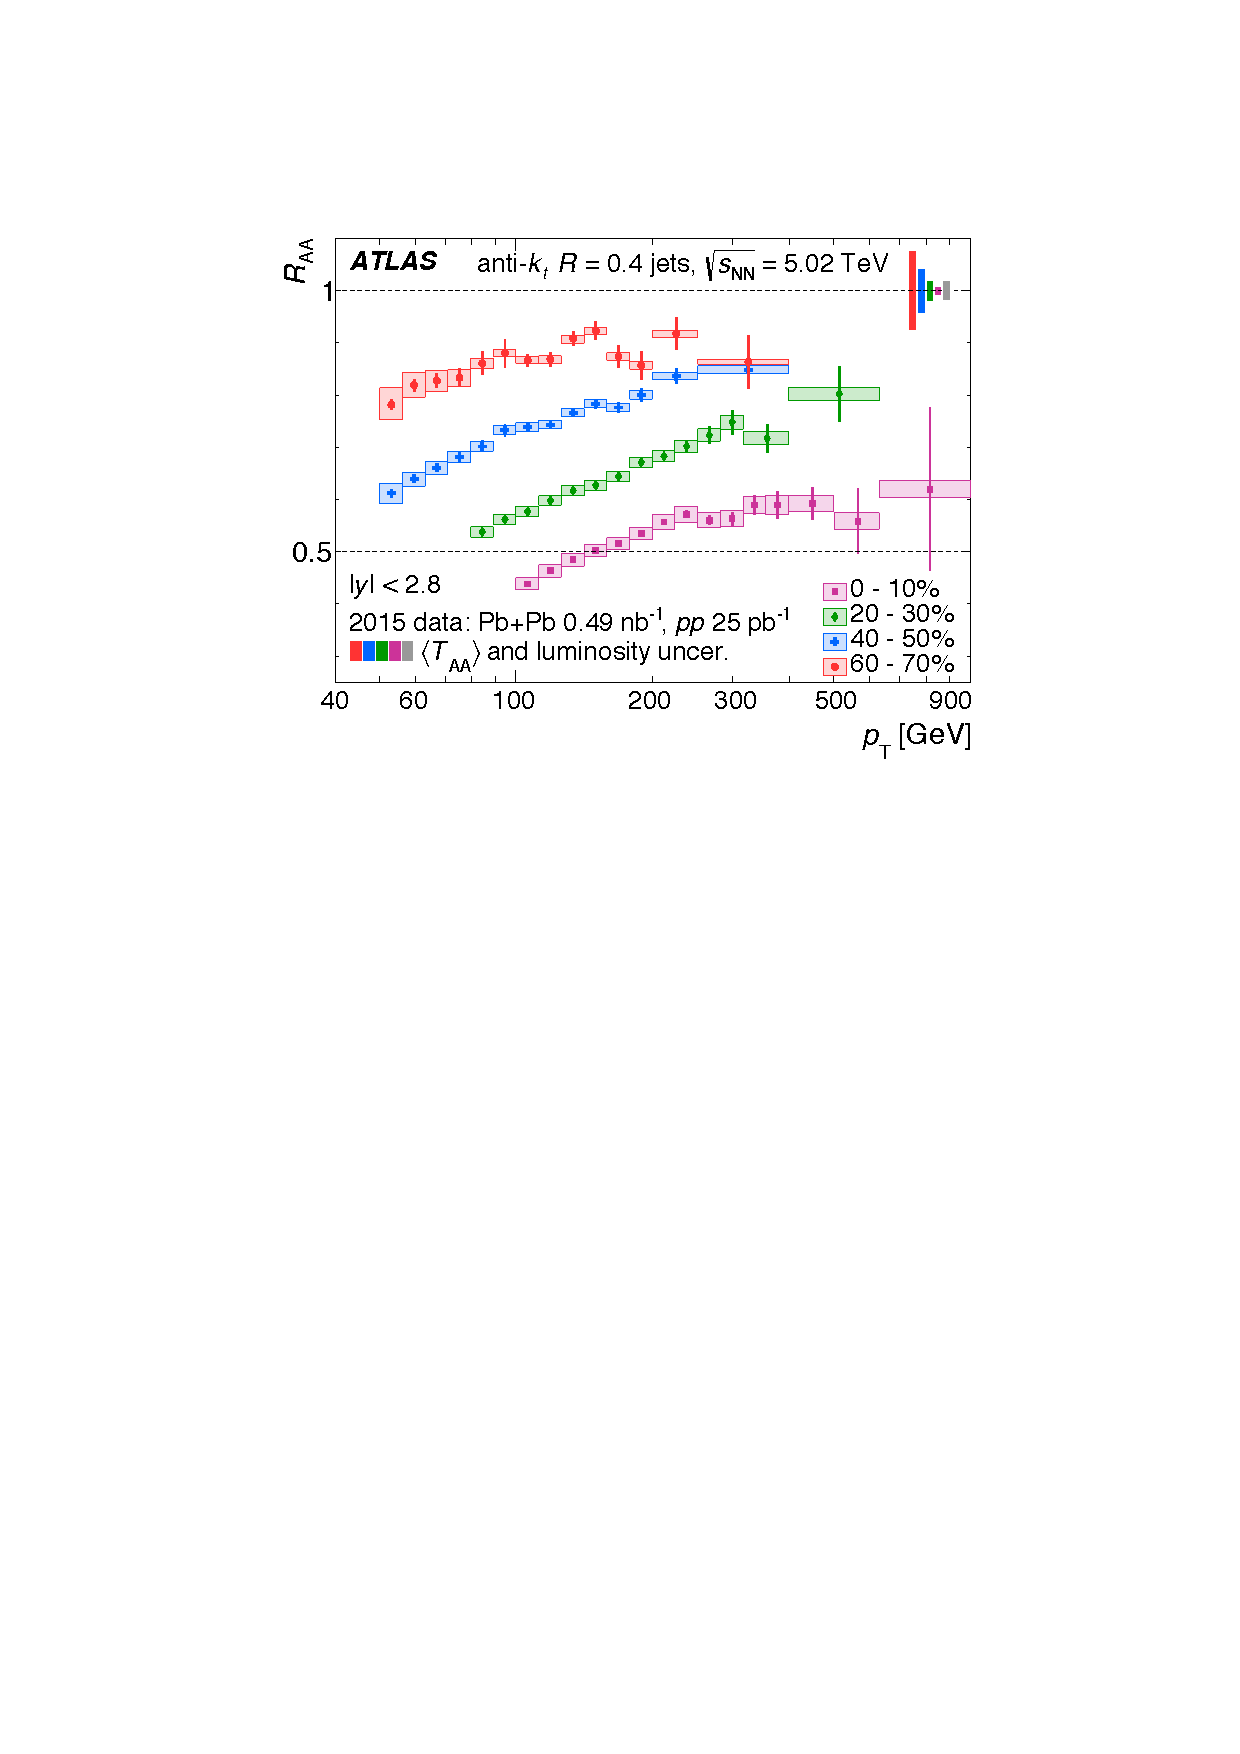
\includegraphics[width=\textwidth]{figures/jetMeasurements/raa}
%\caption{The \RAA\ distributions as a function of jet \pt\ for different centrality bins and jet rapidity $|y| < 2.8$.
%The error bars represent statistical uncertainties while the shaded boxes represent systematic uncertainties.
%Figure taken from \cite{2019108}.}
%\label{fig:raa}
%  \end{minipage}
% \qquad  \qquad  \qquad
%  \begin{minipage}[b]{0.43\textwidth}
%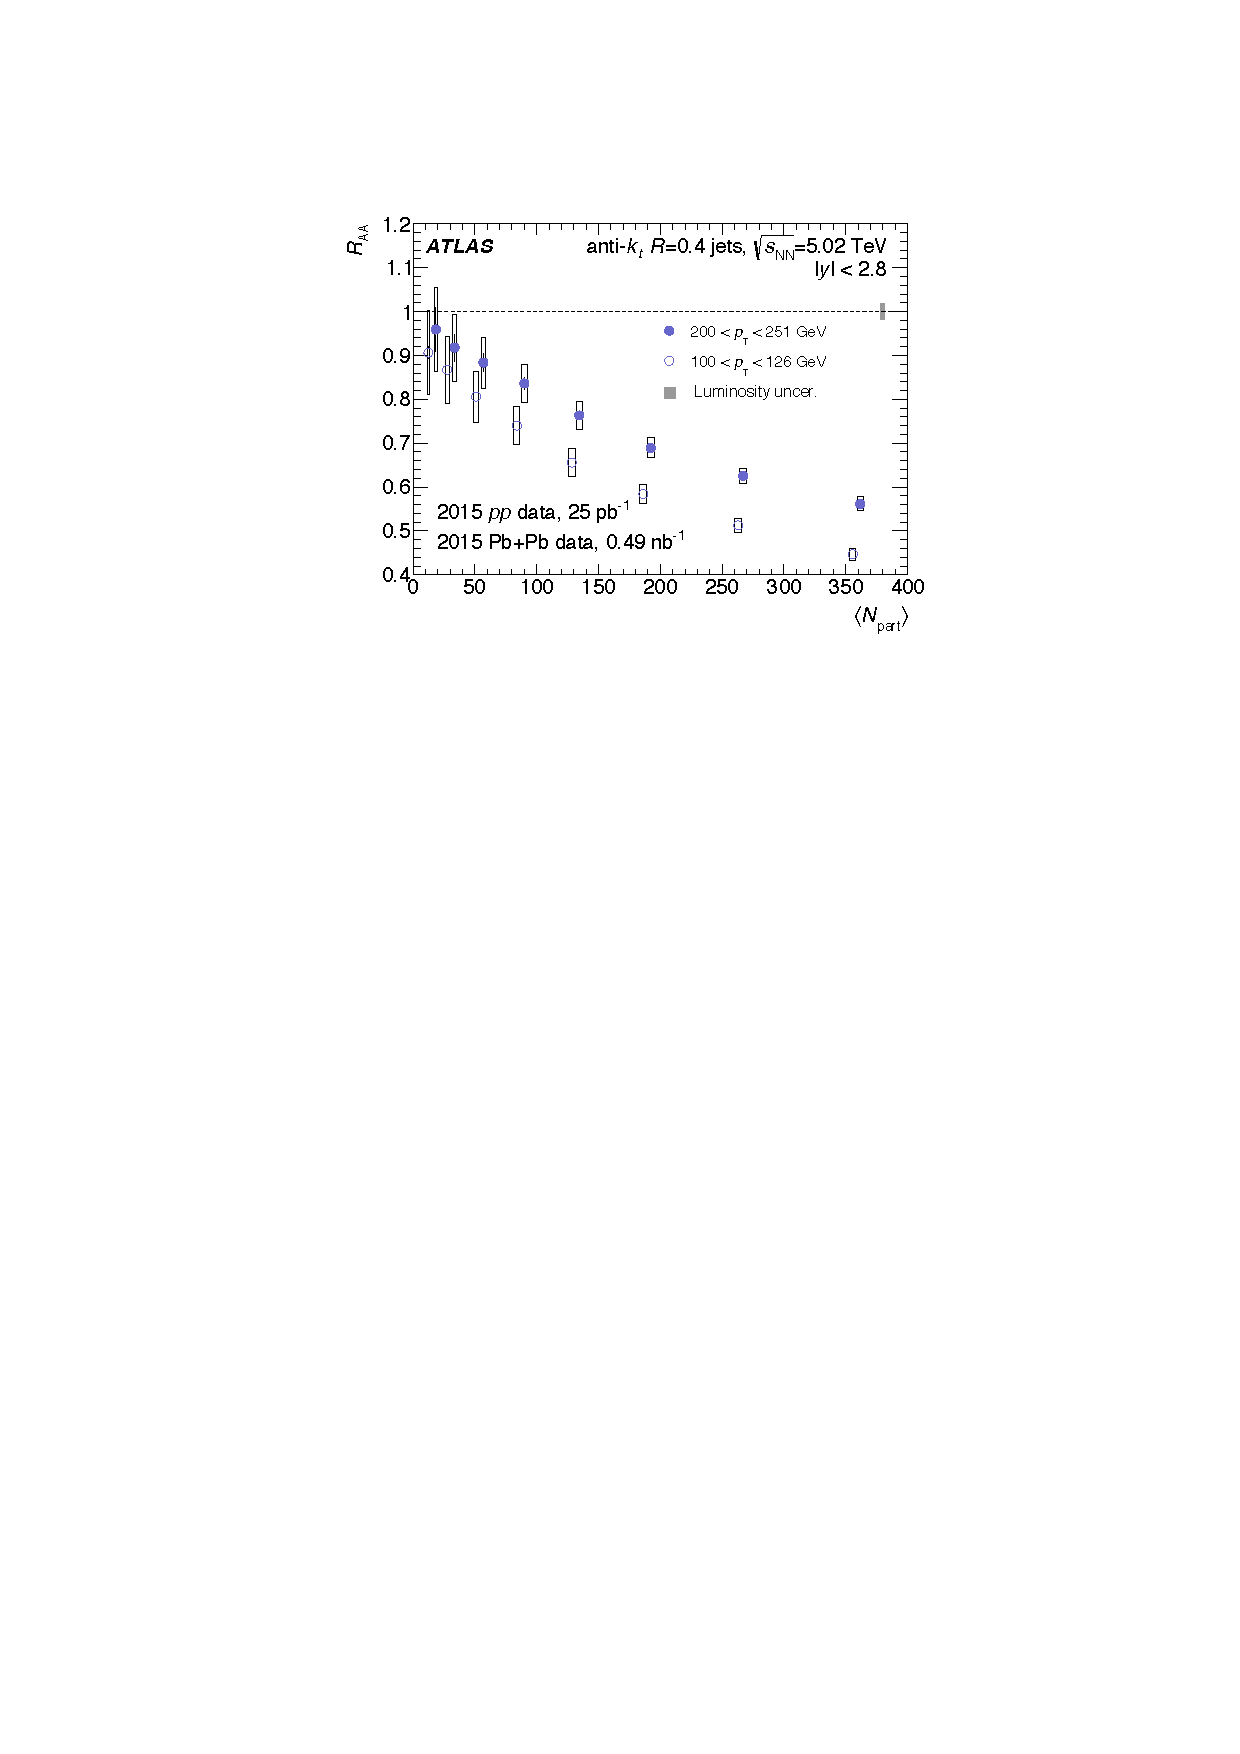
\includegraphics[width=\textwidth]{figures/jetMeasurements/raa_centDep}
%\caption{The \RAA\ distributions as a function of jet \pt\ for different centrality bins and jet rapidity $|y| < 2.8$.
%The error bars represent statistical uncertainties while the shaded boxes represent systematic uncertainties.
%Figure taken from \cite{2019108}.}
%\label{fig:raa_centDep}
%  \end{minipage}
%  \end{center}
%\end{figure}

%
%\begin{figure}[htbp]
%\begin{center}
%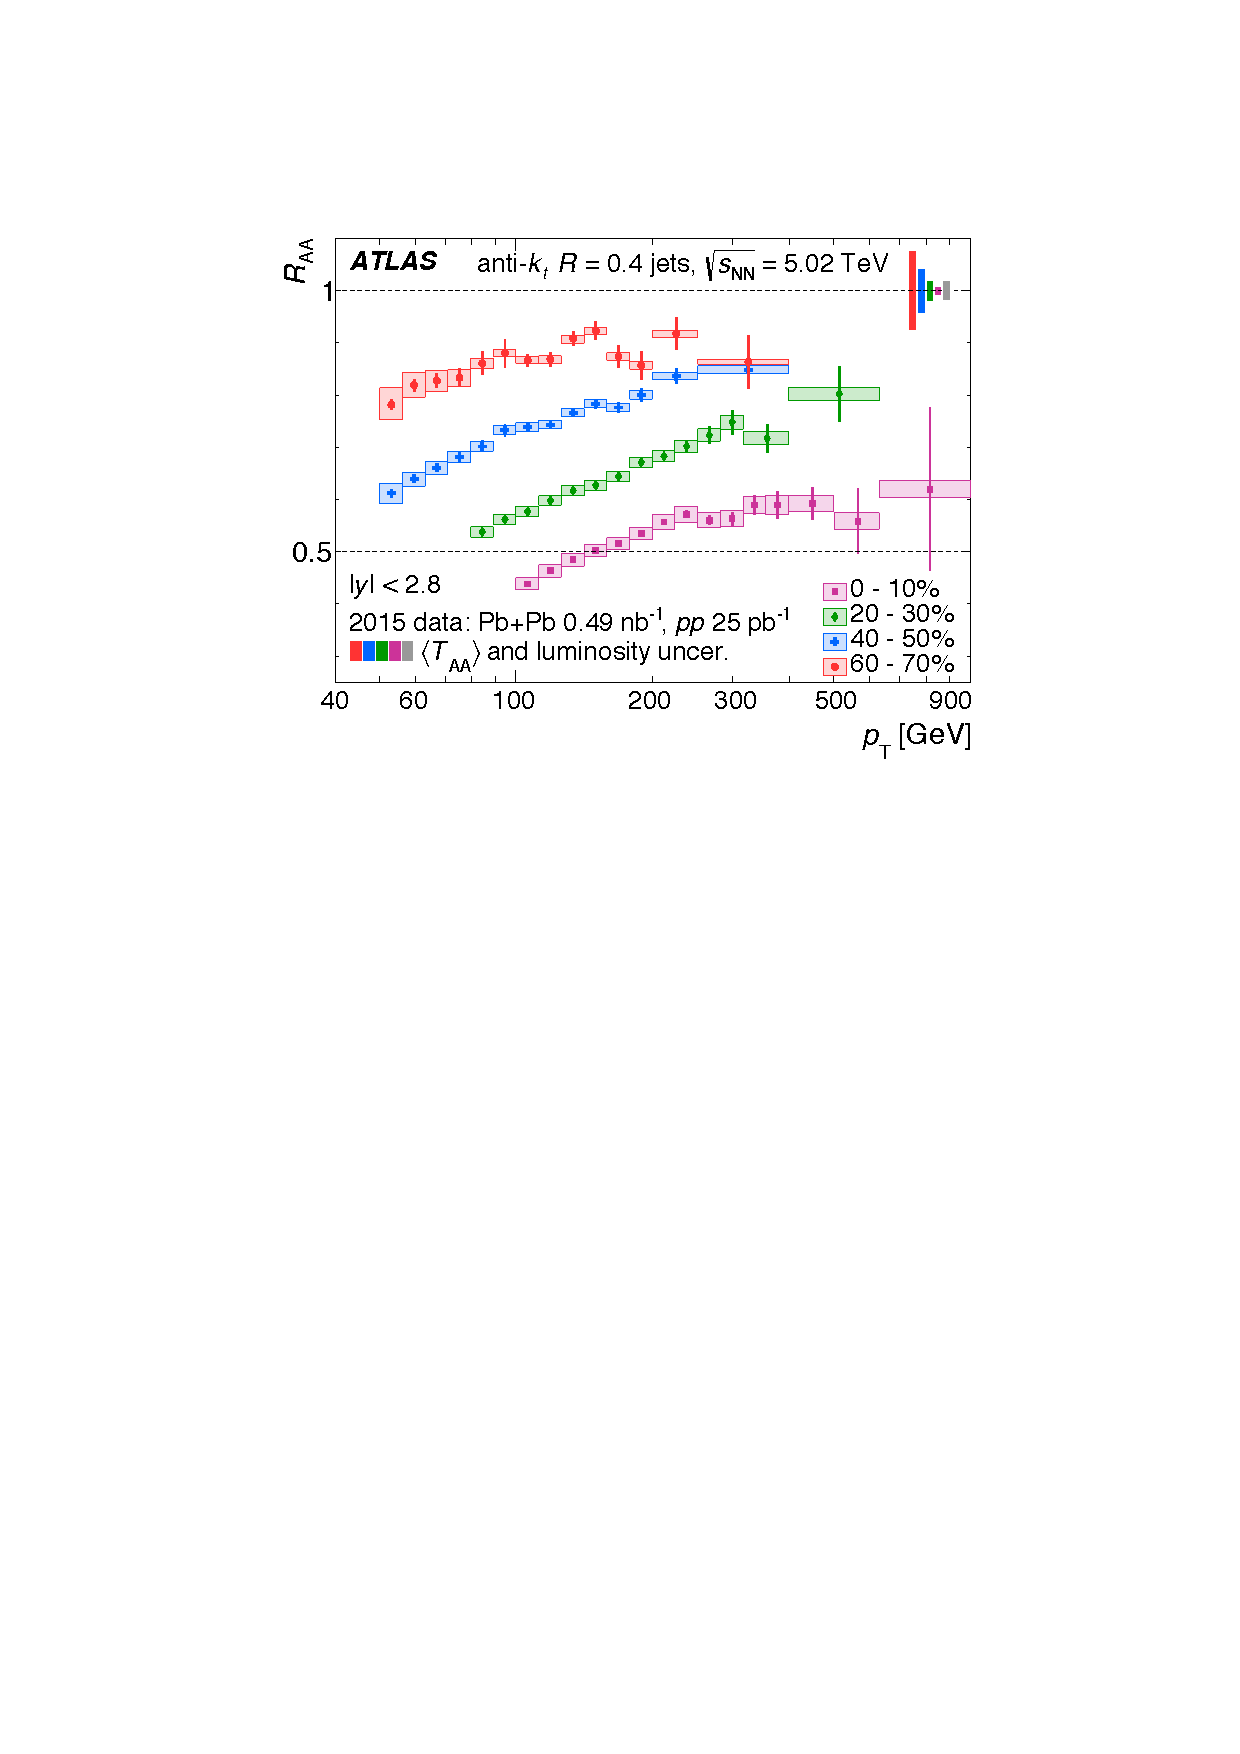
\includegraphics[width=0.55\textwidth]{figures/jetMeasurements/raa}
%\caption{The \RAA\ distributions as a function of jet \pt\ for different centrality bins and jet rapidity $|y| < 2.8$.
%The error bars represent statistical uncertainties while the shaded boxes represent systematic uncertainties.
%Figure taken from \cite{2019108}.}
%\label{fig:raa}
%\end{center}
%\end{figure}


%\begin{figure}[htbp]
%\begin{center}
%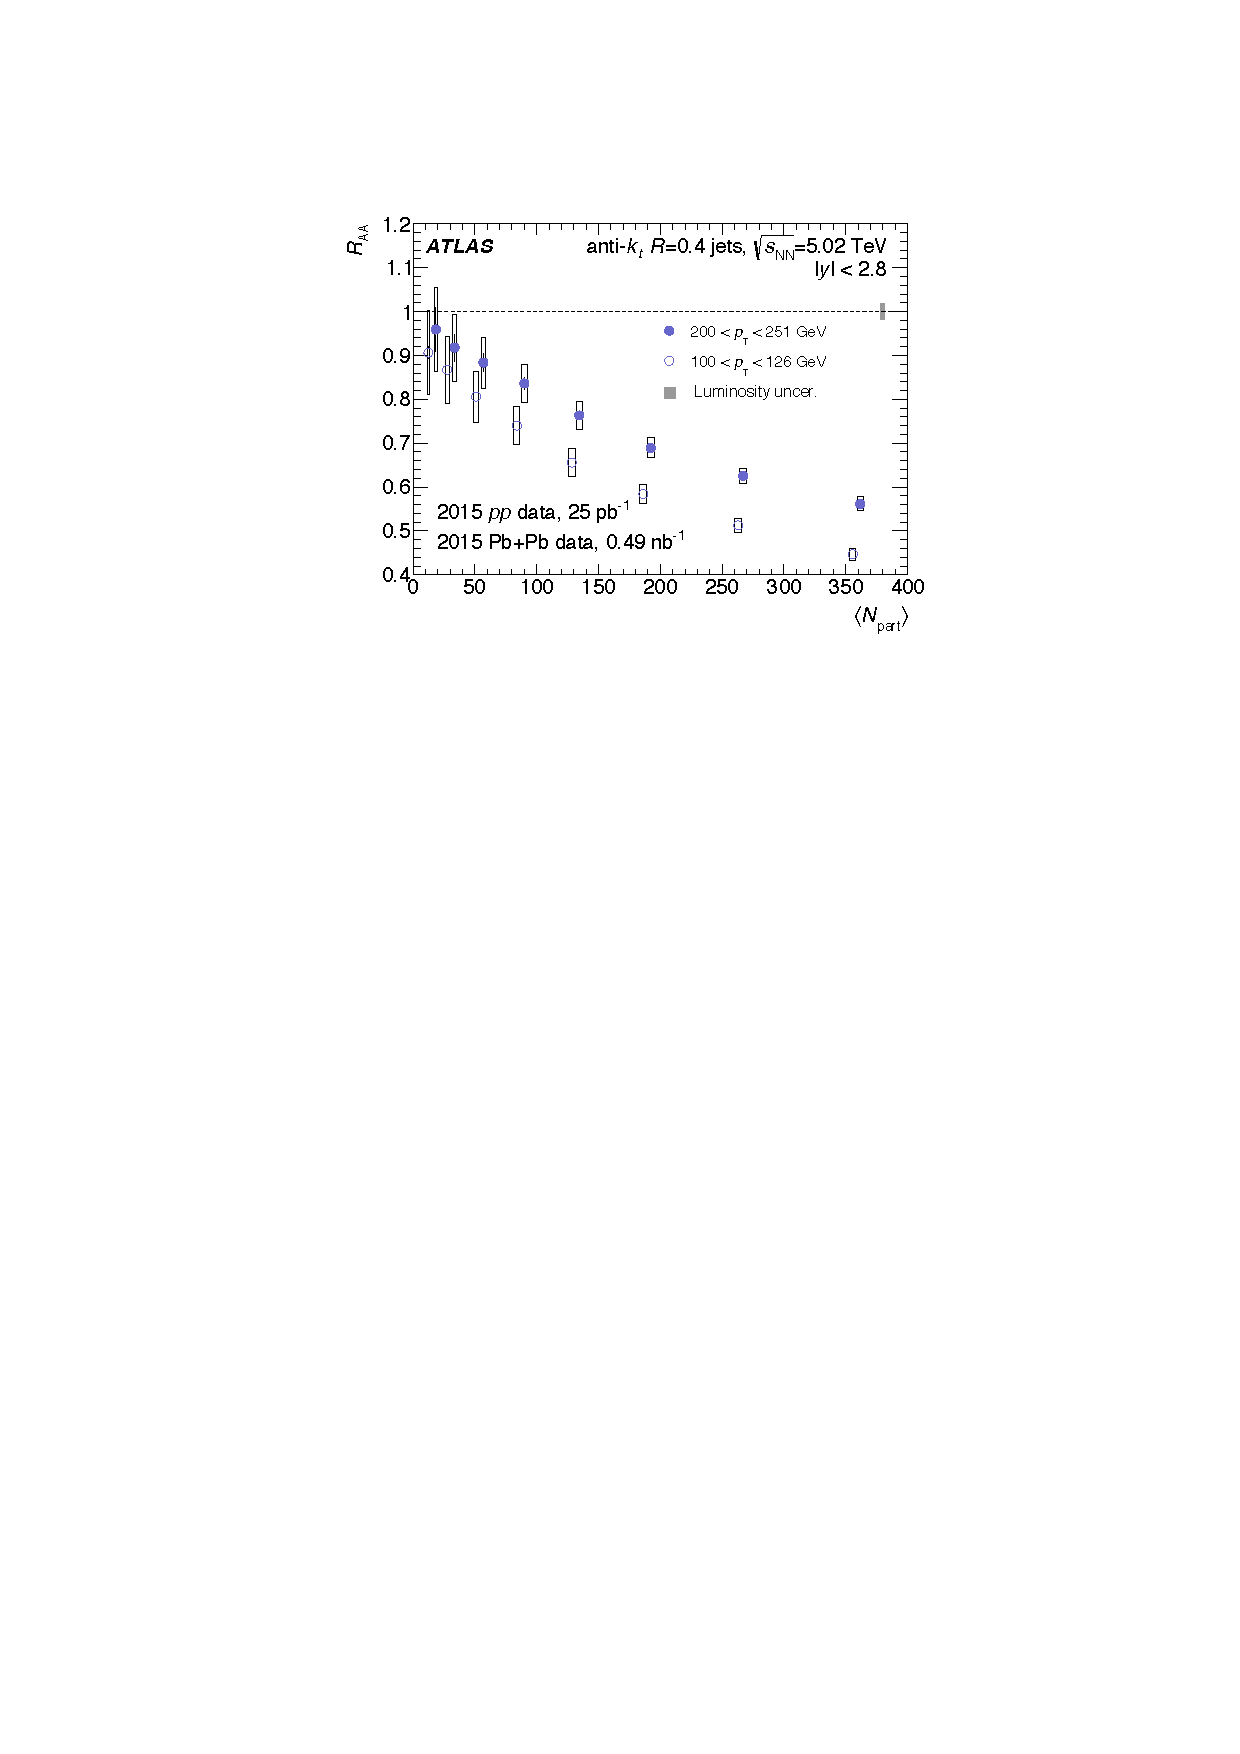
\includegraphics[width=0.55\textwidth]{figures/jetMeasurements/raa_centDep}
%\caption{The \RAA\ distributions as a function of jet \pt\ for different centrality bins and jet rapidity $|y| < 2.8$.
%The error bars represent statistical uncertainties while the shaded boxes represent systematic uncertainties.
%Figure taken from \cite{2019108}.}
%\label{fig:raa_centDep}
%\end{center}
%\end{figure}

%The measurement further looked at the $y$ dependence of \RAA\ as described by $\RAA (|y|) / \RAA (|y| < 0.3)$.
%This is useful because it is sensitive to the different quark to gluon fractions at different rapidities.
% the uncertainties largely cancel, an



